\subsection{Or2yw Tool}
The or2yw toolkit could generate three modes; Yesworkflow is used to construct the JSON-format OpenRefine recipe into the data cleaning diagram. OpenRefine transformations will be extracted as a process. The corresponding values of parameters in transformations are as input parameters in the Yesworkflow system. We provide three modes, including sequential mode, parallel mode, and merge mode. The sequential mode is by following the OpenRefine recipe, step by step. Compared with Sequential mode, the parallel mode would be closer to the dependency relationship among transformations in OpenRefine. Taken the differences of dependencies between columns and inter the same column into consideration, we introduce this "parallel" conception into the data cleaning workflow. In other words, Given a transformation T{$_1$} on column C{$_1$}, if the afterward transformation T{$_x$} also works on column C{$_1$}, then this following transformation is supposed to be dependent on the effect of T{$_1$}. In this situation, the structure of T{$_x$} and T{$_1$} would be sequential. On the other side, if the transformation  T{$_x$} applies to a different column, named column C{$_2$}. As the column C{$_2$} is independent of column C{$_1$}, the  T{$_x$} should be independent with the effect of T{$_1$}, and the structure of T{$_x$} and T{$_1$} would be parallel. With this dependency recovery, the data cleaning workflow in OpenRefine would be much more transparent. As defined in Data Transformation Algebra, Geometry transformation in openRefine would "break" the existing dependency relationships by creating new columns or deleting old columns \cite{nunez2020first}. To get the full provenance information on some column, especially the single cell's provenance, we need to make the dependency information in the data cleaning workflow explicit. 


\subsection{Hybrid Provenance}
We propose a hybrid provenance to fix the transparency and dependency issues with OpenRefine recipe \cite{li2019towards}. There is a $workspace$ in OpenRefine architecture, which has metadata file, and complete provenance files, including $data.txt$ and $history$ folder. 

Provenance information in OpenRefine recipe is the subset of provenance in $data.txt$, for the missing provenance information is recorded in $data.txt$, e.g., the single edit transformation is not recorded in OpenRefine recipe; the other significant extra provenance information provided by $data.txt$ is the history ID, created when data transformation is applied, and the time stamp when processes this transformation.  Thus, we could infer from provenance in $data.txt$ as $P_\mathcal{D}$ to provenance in OpenRefine Recipe $P_\mathcal{OR}$.

\begin{equation}
    P_\mathcal{D} \mapsto P_\mathcal{OR}
\end{equation}

The granularity of provenance information in $data.txt$ and $history$ folder is different; the preceding is of schema level, the succeeding is of cell level. For the missing provenance on the cell level, such as \textit{Single-Edit} transformation, $history$ records the row index, column index, old value, and new value.
For transformations which might bring up dependency broken issues, e.g. \textit{Split-Column} transformation, $history$ records the new generated columns,both values and fields names. Generally speaking, $history$ could fix the partial transparency issues as well as dependency issues. The partial here is because $data.txt$ will record the prospective provenance of transformations, namely transformation function types, function methods, function parameters, while $history$ does not log provenance information that is mandatory for achieving reproducibility and transparency. 

The sharing information between $data.txt$ and $history$ folder is the history ID. We choose to amalgamate the provenance both at $data.txt$ and $history$ through pairing provenance from two ends by history ID, where we named it hybrid provenance. Here provenance in $history$ is rewritten in JSON format following the data types in $data.txt$. JSON is easily readable both for human and machine, uncomplicated for tracing. Then we did several queries on this hybrid provenance to promise its extended transparency, reputability, and completeness \ref{fig:hp_archi}. 

\begin{figure}
\centering
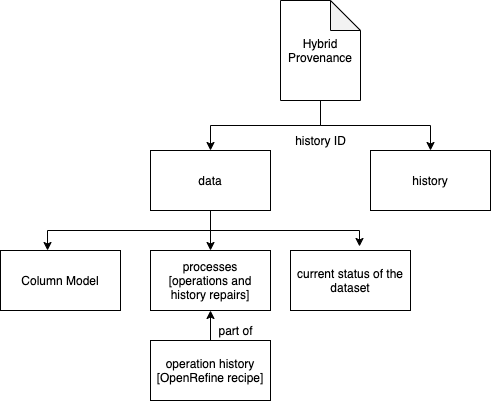
\includegraphics[width=8cm]{Figure/hybrid_provenance_archi.png}
\caption{Architecture of hybrid provenance}
\label{fig:hp_archi}
\end{figure}